\documentclass{article}
\usepackage[utf8]{inputenc}
\usepackage[english]{babel}

\title{TPA - Trabalho 3}
\author{Edson Boldrini}
\date{IFES Campus Serra - 2019/2}

\usepackage{natbib}
\usepackage{graphicx}
\usepackage{minted}
\usepackage{indentfirst}

\begin{document}
\maketitle

\section{Introdução}
Antes de começar a falar sobre o relatório gostaria de informar que minha dupla nesse trabalho era o aluno Caio Kinupp, porém ele não contribuiu com esse trabalho, por isso apenas o meu nome (Edson Boldrini) consta como autor desse documento e autor das soluções dos problemas. 
\par
Este documento tem como objetivo apresentar um relatório sobre as soluções de problemas escolhidos dentro do UVA Online Judge. Estas soluções compreendem o uso e aprendizado de várias estruturas de dados abordadas durante o segundo semestre (2019/2) da disciplina de Técnicas de Programação Avançada ministrada pelo professor Jefferson Oliveira Andrade no IFES Campus Serra.
\clearpage

\section{UVA Submissions}
\begin{figure}[h]
    \centering
    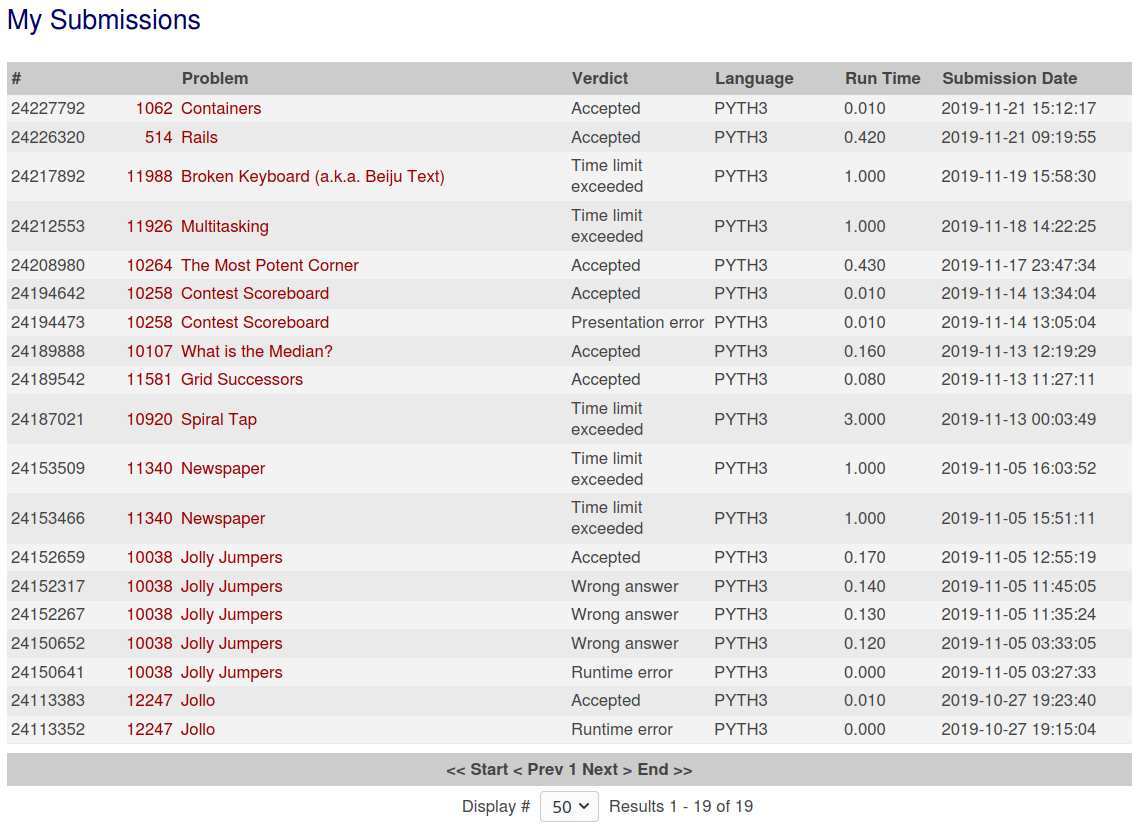
\includegraphics[width=\textwidth]{submissions.png}
    \caption{Submissions}
    \label{fig:submissions}
\end{figure}

Para os problemas 11340, 10920, 11926, 11988 o tempo limite de execução foi excedido, porém arquivos de testes com dados de testes do debug do UVa foram adicionados aos arquivos do trabalho comprovando a eficácia dos algorítmos.

\clearpage

\section{Estruturas de dados}
\subsection{Warm up}
\subsubsection{UVa 12247 – Jollo}
Este problema tem o objetivo de determinar qual a última carta que o príncipe necessita receber para ganhar da princesa não importando quão mal ele jogue. Para chegar a essa solução, desenvolvi um algoritmo que sempre faz com que o príncipe execute a pior jogada possível, ou seja, jogue sempre a maior carta dele menor que a carta que a princesa jogue. Com isso, consigo saber se é possível ele chegar a última rodada tendo ganhado ao menos um dos games (já que estamos numa melhor de 3), caso ele não ganhe nenhum a resposta é -1 pois já terá perdido o jogo, para o caso dele ter ganho ao menos um dos games, a carta que ele necessita receber para garantir a vitória é a carta com o valor da última que sobrou da princesa + 1, verificando se a carta já não saiu antes, caso já tenha saído, incremente até encontrar uma carta que não tenha saído e seja menor que 52.
\inputminted[
frame=lines,
framesep=2mm,
baselinestretch=1.2,
bgcolor=white,
fontsize=\footnotesize,
linenos
]{octave}{uva12247.py}

\subsection{Vetores}
\subsubsection{UVa 10038 – Jolly Jumpers}
Este problema tem objetivo de encontrar sequencias do tipo jolly jumpers. Para encontrar essas sequencias meu raciocínio foi primeiramente encontrar as diferenças permitidas (allowedDifferences) para aquela sequencia de entrada e depois comparei se as diferenças encontradas eram permitidas, caso fossem eu printava "Jolly" e se não fossem printava "Not jolly" assim como a especificação determina.
\inputminted[
frame=lines,
framesep=2mm,
baselinestretch=1.2,
bgcolor=white,
fontsize=\footnotesize,
linenos
]{octave}{uva10038.py}
\subsubsection{UVa 11340 – Newspaper}
Este problema tem o objetivo de encontrar o preço das letras a ser cobrado pela publicação no jornal. Para essa solução, li os dados de entrada sobre os custos de cada caractere e os guardei num dicionário (chave, valor) e após isso caminhei por todo o texto analisando caractere a caractere buscando seu preço definido pelo dicionário anteriormente descrito
\inputminted[
frame=lines,
framesep=2mm,
baselinestretch=1.2,
bgcolor=white,
fontsize=\footnotesize,
linenos
]{octave}{uva11340.py}

\subsection{Matrizes}
\subsubsection{UVa 10920 – Spiral Tap}
Este problema tem o objetivo de saber a posição exata de um determinado número dentro de um tabuleiro espiral. Ao receber o tamanho do tabuleiro e o número para ser encontrado, é determinado em qual quadrante ele está ou seja, em qual dos circulos internos ao tabuleiro ele se encontra. Após determinar o quadrante em que ele se encontra o número é procurado pela linha e coluna utilizando duas variáveis auxiliáres (lb = lowerbound e pad = padding) para encontrar o limite inferior de busca e a quantidade de quadrantes fora dali, com essas duas variáveis é possível determinar a linha e a coluna do número encontrado utilizando elas para caminhar entre as posições possiveis.
\inputminted[
frame=lines,
framesep=2mm,
baselinestretch=1.2,
bgcolor=white,
fontsize=\footnotesize,
linenos
]{octave}{uva10920.py}
\subsubsection{UVa 11581 – Grid successors}
Este problema tem o objetivo de informar qual o índice que permite que a função aplicada a matriz retorna uma matriz com 0 em todas as posições. Para achar a solução deste problema é definido dois arrays auxiliares para comparações, dx e dy. Com esses arrays auxiliares é possível convertendo a matriz em cada execução, quando ela chega a zero, o programa termina.
\inputminted[
frame=lines,
framesep=2mm,
baselinestretch=1.2,
bgcolor=white,
fontsize=\footnotesize,
linenos
]{octave}{uva11581.py}

\subsection{Ordenação}
\subsubsection{UVa 10107 – What is the Median?}
Este problema tem objetivo de encontrar a mediana de uma cadeia de números a medida que ela cresce. Para resolver esse problema o array foi ordenado a cada inserção e depois o tamanho dele foi usado para descobrir a posição da mediana. Caso o tamanho do array seja ímpar, a posição da mediana é exatamente o meio do array, caso seja par, a mediana é a média entre as duas posições mais ao centro do array.
\inputminted[
frame=lines,
framesep=2mm,
baselinestretch=1.2,
bgcolor=white,
fontsize=\footnotesize,
linenos
]{octave}{uva10107.py}
\subsubsection{UVa 10258 – Contest Scoreboard}
Este problema tem objetivo de encontrar o score final de um torneio de programação. Para encontrar essa solução foram utilizados dois dicionários auxiliares, um de submissões corretas e outro submissões incorretas, para assim calcular as pontuações corretas de cada competidor. Cada linha (submissão) é processada unicamente e calcula a pontuação ou penalidade referente a aquela submissão.
\inputminted[
frame=lines,
framesep=2mm,
baselinestretch=1.2,
bgcolor=white,
fontsize=\footnotesize,
linenos
]{octave}{uva10258.py}

\subsection{Manipulação de bits}
\subsubsection{UVa 10264 – The Most Potent Corner}
Este problema tem o objetivo de encontrar a vizinhança (aresta) do cubo que tem a potência mais alta. Para encontrar essa aresta mais potente são calculadas as potências de todos os vértices e a partir daí encontrar dentre essas potências, a aresta mais potente (os dois vértices vizinhos que somados tem a maior potência). Após ser encontrado, esse valor da potência é printado.
\inputminted[
frame=lines,
framesep=2mm,
baselinestretch=1.2,
bgcolor=white,
fontsize=\footnotesize,
linenos
]{octave}{uva10264.py}
\subsubsection{UVa 11926 – Multitasking}
Este problema tem objetivo determinar se as tarefas planejadas de uma pessoa tem conflito de horário ou se não tem. Para resolver esse problema transformei as tarefas repetitivas em tarefas de execução única, trazendo as tarefas repetitivas para a linha to tempo de tarefas de execução única definindo como elas se comportariam no contexto de tarefas de execução única. Após isso, é verificado se na linha do tempo gerada as tarefas tem conflito ou não, inserindo uma a uma até a finalização da lista de tarefas.
\inputminted[
frame=lines,
framesep=2mm,
baselinestretch=1.2,
bgcolor=white,
fontsize=\footnotesize,
linenos
]{octave}{uva11926.py}

\subsection{Lista Encadeada}
\subsubsection{UVa 11988 – Broken Keyboard (a.k.a. Beiju Text)}
Este problema tem objetivo de mostrar qual é o texto final gerado pela digitação de um usuário com problema no teclado. Para essa solução foi pensado uma variável chamada "cursor" que faz o papel de escrever o caractere que veio da lista de entrada no novo texto na posição que a variável cursor informa. Cursor é incrementado em 1 para que o texto possa seguir o fluxo em frente quando não há erros do teclado, representados pelos caracteres "[" (keyboard home button) e "]" (keyboard end button).
\inputminted[
frame=lines,
framesep=2mm,
baselinestretch=1.2,
bgcolor=white,
fontsize=\footnotesize,
linenos
]{octave}{uva11988.py}

\subsection{Pilhas}
\subsubsection{UVa 00514 – Rails}
Este problema tem objetivo de informar se é possível reorganizar os vagões da estação de trem. É um programa simples de pilha onde caso a pilha de trens na estação esteja vazia ao fim das organizações significa que é possível (print "Yes", do contrário, não é possivel (print "No").
\inputminted[
frame=lines,
framesep=2mm,
baselinestretch=1.2,
bgcolor=white,
fontsize=\footnotesize,
linenos
]{octave}{uva00514.py}
\subsubsection{UVa 01062 – Containers}
Este problema visa calcular quantas pilhas são necessárias para poder carregar as embarcações por ordem alfabética. É um outro programa simples de pilha que aloca uma pilha nova cada vez que uma letra nova que ainda não tem sua pilha alocada aparece na sequência.
\inputminted[
frame=lines,
framesep=2mm,
baselinestretch=1.2,
bgcolor=white,
fontsize=\footnotesize,
linenos
]{octave}{uva01062.py}

\end{document}